\chapter{State-of-the-art}
\label{sec:stateoftheart}

%\footnote{The name of this thesis is about processing of medical information. Processing of any type of information might be done using local PC. The processing might take a lot of time thus it's desirable to perform processing on some more powerful hardware: workstation, server, cluster of servers.}

The processing of medical information deals with methods that connect different scientific domains, computer science, biomedical engineering and medicine, together with a common goal. 

%Medical informatics, computational biology, bioinformatics}
%Medical informatics (MI)\nomenclature{MI}{Medical informatics} 
%deals with informatics methods used in clinical medicine and healthcare. While bioinformatics %(BI)\nomenclature{BI}{Bioinformatics} 
%focus more on development and application of new informatics techniques in biological (mainly genomic) sciences. Computational Biology % (CB)\nomenclature{CB}{Computational biology}
%study the biological systems formalized as mathematical models and using computational methods to simulate and compare with real systems. Recent development in the medical informatics and bioinformatics joined a scientific effort to translate the successful techniques from bioinformatics into clinical medicine and healthcare as well as to improve related scientific disciplines in medicine as well in informatics or computer science.
%Maojo et al. \cite{Maojo2003} and Martin-Sanchez et al.\cite{Martin-Sanchez2004} described relationship between medical informatics and bioinformatics to determine a new domain of biomedical informatics.

%Further chapters touch the approach to develop new techniques in informatics inspired from genetic and biology and deliver such techniques to clinical use or basic research within the field of computational biology.

From a computer science (informatics) point of view, it is assumed that the processing of medical information is, in general, a computational problem, which is understood as a task that can be solved by a computer. 

As some computationally hard problems ar discussed later in this thesis, the next sections briefly introduce the theoretical and practical aspects, as well as the consequences, of theory of computation, parallelism and distributed computing. Section \ref{sec:introcomplexity} introduces some of the important complexity classes of problems from the view of the computational complexity theory. 

Parallel computation can introduce speedup of computation when specific conditions are fulfilled. This theory is briefly covered in section \ref{sec:introparalel}.

The distribution of a parallel task via a computer network to other computers, servers and cluster of servers is covered in section \ref{sec:distributed}, with a focus on grid computing and cloud computing.

\section{Computational Complexity}
\label{sec:introcomplexity}

An algorithm is a set of operations that is used to accomplish tasks and solve problems. There are several ways of expressing algorithms, e.g., in text, in programming language, pseudo-code or flowcharts. Later in this thesis kopenograms will be used as a graphical language for structured algorithms in order to supplement the Unified Modeling Language (UML) diagrams\nomenclature{UML}{Unified Modeling Language}, as proposed by Kofranek et al.\cite{Kofranek2012}\footnote{\url{http://www.kopenogram.org} accessed March 2015}.

The computational complexity theory classifies problems into several classes, according to the time or space needed by the algorithm in order to solve the problem. The time complexity of an algorithm is usually denoted by a big $O$ notation and size of input problem $n$ meaning that a time complexity denoted by $O(g(n))$ is not growing faster than the function $g$. Formally $f(n)=O(g(n))$, if, and only if, there is a constant $c$ and positive integer $n_0$ that for each $n\geq n_0$: $f(n) \leq c \times g(n)$.

$O(1)$ denotes algorithms that take constant time, regardless of the input size. $O(n)$ denotes linear time algorithms, i. e., time is linearly dependent of the input size. For example, figure \ref{fig:search} shows the sequential search algorithm in a pseudo-code and kopenogram, which needs to compare each record with a given key. This is used to find some items in an unsorted list or array. For example, if a single comparison takes $0.03$ seconds and the list has $n$ records, then the algorithm will take, at worst, $n$ steps and the time complexity will be $f(n) = 0.03 \cdot n = O(n)$. \footnote{A search problem can be solved by the sequential search algorithm, which is a brute force approach that tries all of the values. There are better approaches for a search problem, e.g., a binary search algorithm on a sorted list, taking logarithmic time complexity $O(\log(n))$, which outperforms the sequential search. B-trees are the most used structure for holding the sorted list of elements in production application or databases\cite{Bayer1972Org,Bayer1972Sym}.}

\vspace{10mm} % to keep further pages unchanged

\begin{figure}[ht]
    \centering
    \includegraphics[page=3]{chapter3/GA-kopenogram2-crop.pdf}    
%    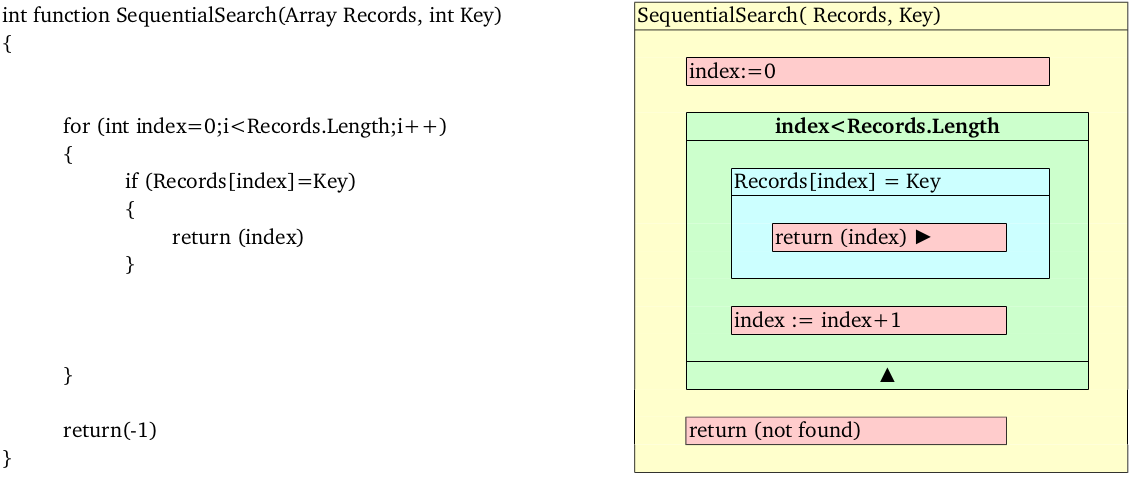
\includegraphics[width=1\textwidth]{chapter2/seqsearchkopenogram.png}
    \caption{Pseudo-code (left) and kopenogram (right) of a sequential search algorithm with the time complexity $O(n)$. The red blocks are commands, i.e., setting the index or returning results. The green block represents the loop with entry condition. The index is incremented and in programming languages this is achieved by, e.g., \emph{for} cycle statement. The blue block is the condition (\emph{if} statement). When this is fulfilled, then the inner blocks are executed and, in our case, the found index is returned. If no record is found, the loop will end with the last index within \emph{Records} and \emph{not found} sign is returned.}
    \label{fig:search}
\end{figure}

Polynomial time algorithms are defined as the ones that time complexity is bound by $O(n^k)$ for some constant $k$. The class of problems, solvable by polynomial algorithm, is denoted as \emph{class P} and is recognized as tractable -- first noted by Cobham and Cook \cite{Cobham1964,Cook1983}. Other algorithms, whose time cannot be bound by any polynomial functions, are called exponential. These are recognized as generally intractable, as published by Garey and Cook \cite{Garey1979,Cook1983}. For a relatively small input data, the exact solution can be found using the known exponential algorithm with a current computation power. However, for bigger input data, the time needed to solve the problem is far a beyond reasonable amount, as seen from Table \ref{table:timecomplexity}.

A class \emph{NP-complete} of hard problems was identified where it is not known whether a polynomial time algorithm exists, i.e., whether they belong to \emph{class P}. 
To find a solution for such problems, the current best-known class of algorithm is based on a brute-force search of all of the possible values, which suffers with exponential time complexity $O(k^n)$. 
%It is an open question as to whether a better one exists. 
The solution founded by the previous algorithm, can be then verified in polynomial time. 
Additionally, the class of \emph{NP-complete} problems are related; if some polynomial algorithms are found for one of the problems, then a derived algorithm will solve other problems of this class in polynomial time too. 
This feature of \emph{NP-complete} class of problems was denoted by Cook and Karp \cite{Cook1971,Karp1972}. 

A brute-force search is a general solving technique that generates all of the possible candidates of solution and checks if the problem satisfies the problem statement. All brute-force search algorithms suffer with exponential time complexity $O(k^n)$\footnote{For example, depth-first iterative-deepening algorithm for a brute-force search was shown to be optimal, compared to other standard brute-force search algorithms (depth-first search or breadth-first search) \cite{Korf1985,Pearl1987}.}.

%In the past there were identified several class of problems, for which the current 
%For the class of \emph{NP-complete} problems (non-deterministic polynomial, where if some guess is provided, it can be verified in polynomial time whether it is the solution or not) the current 
%best known algorithm is based on brute-force search of all possible values and better does not exists, or it is open question whether it exists. E.g. For the class of {NP-complete} problems if a polynomial algorithm will be discovered for one problem of this class in future, it was shown that all other NP-complete problems would be solvable by a polynomial algorithm derived from the discovered one\cite{Cook1971,Karp1972}.

%The analysis of complexity of algorithms and problems mentioned above is important for further consequences on computability.
\begin{table}[ht]
\footnotesize
\begin{tabular}{|l|r|r|r|r|}
\hline
\diagbox[height=43pt,width=125pt]{time\\complexity\\function}{input size \\ $n$} & 10          & 20        & 50             & 100            \\ \hline
$O(n)$                                                                           & $00.01$ s     & $00.02$ s   & $00.05$ s        & $00.10$ s        \\ \hline
$O(n^2)$                                                                         & $00.10$ s     & $00.40$ s   & $02.50$ s        & $10.00$ s        \\ \hline
$O(n^5)$                                                                         & $01$m $40.00$ s & $53$ m $20$ s & $14$h $48$m $20$s    & $116$ days       \\ \hline
$O(2^n)$                                                                         & $01.02$ s     & $17$ m $28$ s & $35702$ years    & $4.02\times 10^{19}$ years \\ \hline
$O(3^n)$                                                                         & $59.05$ s     & $40$ days   & $2.28\times 10^{13}$ years & $1.63\times 10^{37}$ years \\ \hline
\end{tabular}
\caption{The computation time of algorithms with different time complexity functions, where one step of algorithm takes 1 millisecond. Examples of algorithm with polynomial time complexity $O(n^k)$ are compared to algorithms with exponential time complexity $O(k^n)$. It is important to note that, for the problems with an input size of 50 and greater, the exponential algorithm runs far beyond the reasonable time, compared to, e.g., the age of the universe, which is currently estimated to be $13.8\times 10^9$ years \cite{PlanckCollaboration2013}.}
\label{table:timecomplexity}
\end{table}

If we presume that the technological update and computation speed will increase, the effect of the technological speedup is visible in Table \ref{table:speedupeffect}. The effect on the polynomial algorithm is multiplicative. However, for the exponential algorithm, the technological speedup will only slightly increase the size of the computable problem. This is the reason why the problems solvable by  only exponential algorithm are denoted as intractable. 
\begin{table}[ht]
\footnotesize
\begin{tabular}{r|c|c|c|c|}
                      & present computer   & 10 times faster               & 100 times faster               & 1000 times faster \\
\hline
\multirow{2}{*}{$O(n)$}  & $3\,600\,000$        & $36\,000\,000$         & $360\,000\,000$        & $3\,600\,000\,000$      \\
                      & $1\times$          & $10\times$   & $100\times$  & $1000\times$ \\
\hline
\multirow{2}{*}{$O(n^2)$}                 & $1\,897$ & $6\,000$             & $18\,973$ & $60\,000$            \\
                      & $1\times$          & $3.16\times$ & $10\times$   & $31.6\times$ \\
\hline
\multirow{2}{*}{$O(n^5)$}                 & 20  & 32     & 51    & 81    \\
                      & $1\times$          & $1.59\times$ & $2.51\times$ & $3.98\times$ \\
\hline
\multirow{2}{*}{$O(2^n)$}                 & 21  & 25    & 28    & 31    \\
                      & $N_{2^n}$       & $N_{2^n}+3.32$    & $N_{2^n}+6.64$    & $N_{2^n}+9.97$    \\
\hline
\multirow{2}{*}{$O(3^n)$} & 13  & 15    & 17    & 20    \\
                      & $N_{3^n}$       & $N_{3^n}+2.09$    & $N_{3^n}+4.19$     & $N_{3^n}+6.29$                  \\
                      \hline
\end{tabular}
\caption{Effect of computation speedup. The first value is the input size of data that is computable in one hour and the second value is the speedup that is achieved, compared to the value in first column. }
\label{table:speedupeffect}
\end{table}

%Note that the age of universe is currently estimated to $13.8\times 10^9  years$ \cite{PlanckCollaboration2013}.
\emph{NP-complete} problems are covered in the published works of Garey and Johnson \cite{Garey1979}. The whole complexity theory is also covered in published works of Papadimitriou \cite{Papadimitriou1995} or Sipser \cite{Sipser2012}. 

The technological speedup will mainly impact the class of problems, which are solvable by polynomial algorithm. Other non-exact methods are used to find at least some solution for the problems that are only solvable by exponential algorithms. Examples of these methods are: 
\begin{itemize}
\item{The \emph{heuristic method} tries to eliminate the number of steps of computation by some implicit or explicit knowledge of the specific problem itself, e.g., eliminating solution classes that seem to not go to optimal solution. With a combination of a brute-search, the heuristic method reduces the size of all of the possible solution candidates to check. More can be found in the published works of Russel et al. \cite{Russell2009}}
\item{The \emph{randomization method} uses a non-deterministic methods in some level of computation. For example, the Monte-Carlo method is used to compute problems using pseudo-random generated values and, after several iterations, statistical methods are used to compute the expected value and standard deviation \cite{Manly2007}. }
\item{\emph{Restriction on input data} -- this is another form of using the explicit knowledge of the problem instance and it may reduce all of the possible values to be checked by brute-force search. }
\item{\emph{Approximation algorithm} -- this not only finds some good solutions, but also, it quantifies how far from the optimal solution the result is, with some degree of probability.}
\end{itemize}

\section{Parallelization}
\label{sec:introparalel}

If a sequence of instructions can be divided into parts, which can be computed independently in parallel by multiple processors, then it is possible to achieve some computation speedup using current computational technology. %Parallel computing can be utilized in several types of application which are further distinguished by the types of location and access to the computation resources. 

A speedup of a computation on P processors can be defined as:
\begin{equation}\label{eq:speedup}
 S(P) = \frac{\text{time on 1 processor}}{\text{time on P processors}}
 \end{equation}

%We can estimate speedup of an computation of a fixed-size problem and then we can ask how can we speedup this problem on P processor. 
Figure \ref{fig:serialvsparallel} shows serial and parallel execution computations of the same algorithm.

\begin{figure}[ht]
    \centering
    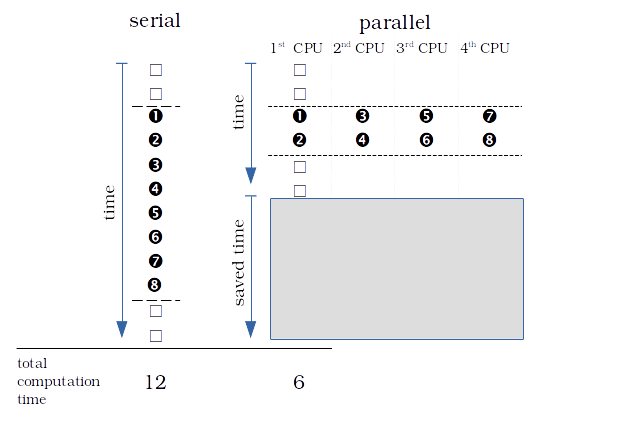
\includegraphics[width=1\textwidth]{serialvsparallel.png}
    \caption{Comparison of serial and parallel executions of instructions. The instructions with numbers can be executed in parallel. In this case, the serial computation takes 12 cycles, parallel computation on four central processing unit(CPU)\nomenclature{CPU}{Central Processing Unit} takes six cycles and the achieved speedup is two. If we have eight CPUs, then the computation will be finished in five cycles (achieved speedup will be $2.4$ times).}
    \label{fig:serialvsparallel}
\end{figure}

Assume $\alpha \in (0,1)$ as a fraction of the computation in one processor, which cannot be parallelized, $(1-\alpha)$ is a fraction of the computation in one processor, which can be parallelized by $P$ processors, and $t$ is the time needed to compute the process on one processor. Assume that the overhead\footnote{Overhead is time spent on communication and synchronization among parallel processes rather than on solving the problem} of parallelization is small and can be disregarded. Then, the speedup can be computed as:
\begin{equation}\label{eq:speedup2}
 S(P) = \frac{t\times\alpha+t\times(1-\alpha)}{t \times \alpha + \frac{t \times (1-\alpha)}{P} } = \frac{1}{\alpha +\frac{1-\alpha}{P}}
 \end{equation}
On an unlimited number of processors, a theoretical upper bound of speedup can be formulated, which depends on $\alpha$ only, denoted as Amdahl's law \cite{Amdahl1967}:
\begin{equation} \label{eq:amdahl}
S = \lim_{P \to \infty} \frac{1}{\alpha +\frac{1-\alpha}{P}} = \frac{1}{\alpha}
\end{equation}

For example, when a 33\% of a computation cannot be parallelized ($\alpha = 0.33$), then the speedup on eight processors can be theoretically $S(8) = \frac{1}{0.33+0.7/8} \dot= 2.4$ and theoretical speedup on unlimited number of processors is $S = \frac{1}{0.33} \dot= 3$. See more in Figure \ref{fig:amdahl}.
\begin{figure}[ht]
    \centering
    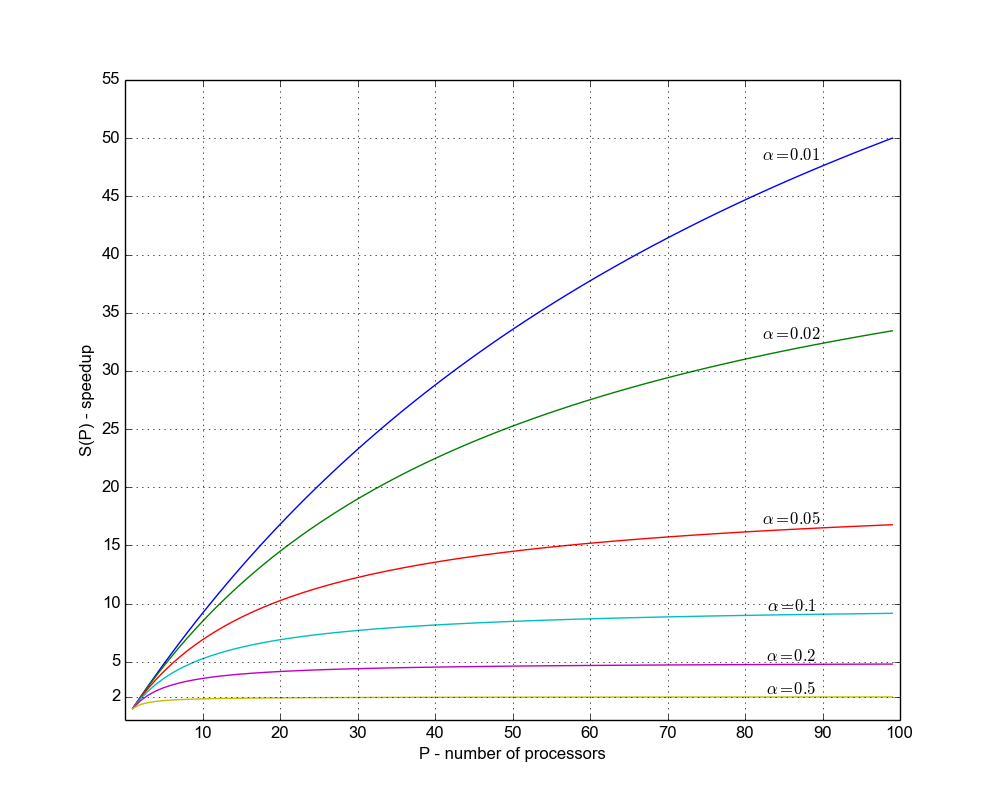
\includegraphics[width=1\textwidth]{chapter2/Amdahl.png}
    \caption{Speedup gained on 1 to 100 processors per Amdahl's law for different $\alpha$ values.}
    \label{fig:amdahl}
\end{figure}

However, $\alpha$ can sometimes be hard to estimate. Additionally, the computing of the fixed size problem on a high number of processors can misrepresent the speedup expectation. Therefore, Gustafson reformulated the law and described another approach -- to measure the fraction of the computation, which cannot be parallelized from computing on $P$ processors. This approach estimates the time of how long will such computation take on single processor and speedup is determind from this estimation. In this case, assume that the overhead of parallelization is small and can be disregarded. The $\beta$ is the "scaled fraction" of the computation on $P$ processors, which cannot be parallelized \cite{Gustafson1988}:
\begin{equation} \label{eq:gustafson}
S(P) = \frac{t \times \beta + t\times(1-\beta)\times P}{t\times\beta+t\times(1-\beta)} = \beta + (1-\beta)\times P 
\end{equation}
This law presumes that the fraction $\beta$ will not change on different number of processors, as seen in Figure \ref{fig:gustafson}.
\begin{figure}[ht]
    \centering
    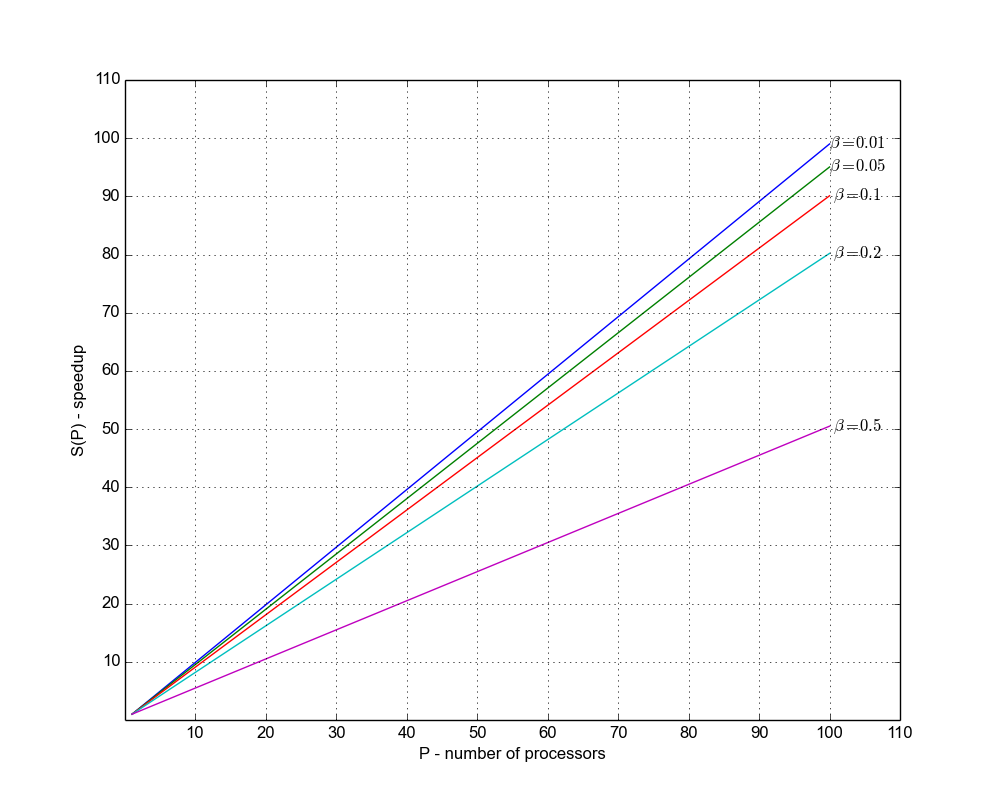
\includegraphics[width=1\textwidth]{chapter2/Gustafson.png}
    \caption{Speedup gained on 1 to 100 processors per Gustafson's law for different $\beta$ values.}
    \label{fig:gustafson}
\end{figure}

Both laws disregard parallelization overhead, however, if there is a significant one, the speedup of parallelization will be degraded by the overhead and can eventually lead to slow down of computation. Amdahl's law (\ref{eq:amdahl}) is argument that maintains the speedup limit for current fixed-sized problems. Gustafson's law, however, is more suitable to estimate speedup for bigger problem size and arguments that problem size scale with parallelization.

\subsection{Programming Model}
\label{sec:parallelprogramming}
There are several levels of how parallelism is realized:
\begin{itemize}
\item{\emph{Instruction level parallelism} -- if the instructions are independent, they can be executed at the same time by a multiple central processing unit(CPU), e.g., by several cores of the multi-core processor. Programs are usually written as a sequence of instructions. Instruction parallelism depends mainly on the compiler's capabilities to recognize or reorder the instruction to execute them in parallel. In the multi-core processor era, instruction parallelism started to be systematically utilized.}
\item{\emph{Data parallelism} -- the same operation is performed on multiple data, usually arrays. The instruction is distributed into multiple processors or processor cores and is executed on elements of data structure in parallel. This is currently the characteristic feature of a computing on \emph{General purpose graphical processing unit}(GPGPU) and programming application interface (API)\nomenclature{API}{Application Interface} such as CUDA\footnote{\url{https://developer.nvidia.com/cuda-zone} accessed February 2015} and OpenCL\footnote{\url{https://www.khronos.org/opencl/} accessed February 2015}}
\item{\emph{Loop parallelism} -- the computation may contain iteration on some large data structures. Such iterative processing is usually programmed as a loop and if $i^{th}$ iteration is independent on previous $(i-1)^{th}$, then the iteration can be executed in parallel by different processors.}
\item{\emph{Task parallelism} -- the computation contains parts that are independent of each other. The computation of such parts can be scheduled and distributed into multiple processors and can be computed concurrently. For example, master/worker pattern is realized by a "master" process which sets up a pool of "worker" processes and a set of tasks is distributed to them. Other example, fork/join pattern is realized by the main process, which forks into several concurent processes doing computation and at some point, they join back into a single process, which may, after some computation, fork again.}
\end{itemize}

Looking at the way the processes interact, these are the most common forms:
\begin{itemize}
\item{The \emph{threads} are several concurrent execution paths that are independent but, in general, share the same memory. They are standardized, e.g., as POSIX threads (Pthreads) and implemented in many platforms. Further reading about Pthreads can be found in the published works of Butenhof \cite{Butenhof1997}. There are also other implementations of the threads going beyond the POSIX standard, which have been introduced in other languages and programming environments.}
\item{\emph{Shared memory}. The \emph{OpenMP}\footnote{\url{http://openmp.org/} accessed February 2015} is a shared memory application interface, which is standardized and implemented by several compilers for programming languages. It also uses a multithreaded model, however, programming is task-oriented and more abstract than using threads, as described by Chapman et al. \cite{Chapman2008}. }
\item{\emph{Message passing}. The \emph{Message Passing Interface}~(MPI)\nomenclature{MPI}{Message Passing Interface} is a specification for performing task communication by passing messages between tasks. Further reading about MPI can be found in the published works of Pacheco \cite{Pacheco1997}.
}
\end{itemize}
More information about parallel programming models can be found in a survey by Diaz et al. \cite{Diaz2012}.

Some algorithms can be easily divided into independent tasks, which can be computed in parallel. If there is minimal or no need to communicate among the parallel tasks, such algorithms are called embarrassingly parallel. For example, 
\begin{itemize}
\item{Operation on matrices  \cite{Moler1986} are currently used to render 2D and 3D graphics.}
\item{Parameter studies, where the same computation is performed using different sets of input parameters \cite{Foster1995}.}
\item{Brute-force search algorithm, where a subset of possible candidates for solution are generated and checked in parallel.}
\item{Genetic algorithm and other evolutionary algorithms \cite{Cantu-Paz1999}.}
\end{itemize}
In contrast to embarrassingly parallel problems, there are problems, which are inherently sequential. Algorithms solving such problems cannot be significantly speeded up by parallel computing. %The theory about this problems and related algorithm which are denoted as problems/algorithm in class \emph{P-complete} are believed not to get significant speedup using parallel computing, see e.g. book of Greenlaw et al. \cite{Greenlaw1995}. 

Both aspects of scalability(speed up gained by parallel computing) and effectivity (time demand based on the size of input data = time complexity) should be considered. Highly scalable algorithms can be outperformed by a sequential algorithm, which solve the same problem with a better time complexity, as noted, e.g., by Madden \cite{Madden2012}. 

Other of parallel computing and the design and build of parallel programs were published in the earlier works of Foster \cite{Foster1995}, D.Culler et al  \cite{Culer1998} or Rauber and Räuder \cite{Rauber2013}. 

\subsection{Summary}

To summarize this section: parallel computing can introduce speedup on current computational technology and some computation problems may become feasible.
Additionally, parallelization overhead and fraction of non-parallelizable parts should be considered as it may degrade the expected speedup.
In the case of exponential algorithm (e.g., for \emph{NP-complete} problems), the speedup will only increase the size of the solvable problem slightly (see Table \ref{table:speedupeffect}) and some problems cannot be (or it is believed that they cannot) significantly speedup by parallel computing. 
Task parallelism and distributed computing will be considered in later text of this thesis.

\section{Distributed computing technologies}
\label{sec:distributed}

%An important idea is to share computational resources among multiple different users and communities. Several issues needs to be addressed e.g. authentication and authorization using security protocols and database of privileges. Other is scheduling, thus the work of all potential users will not collide in one time and in another time the resources will not be utilized. 
Distributed computing is based on the idea of spreading a computation task into a set of computers, which are connected via a computer network.

The main motivations of using distributed computing technologies are to:(1) share, store and exchange resources (2) provide and consume computational services (3) access a much higher capacity of storage and computation than is available locally and (4) connect people.

To manage distributed computing, several challenges are maintained such as synchronization (the exchange of messages in a computation workflow) to achieve, e.g., mutual exclusion (when a task needs exclusive access to some resource), prevent deadlock (no progress is possible) or resource starvation (when resources -- such as processor time -- are not scheduled for a particular task for some reason and the task cannot finish computation). Distributed systems offer some sort of fault tolerance (managing fault of a node during computation) or security (encryption of communicating channels and stored data, authentication and authorization to access some resources or data) etc. The topic of distributed computing is covered in the published works of Tannenbaum \cite{Tanenbaum2007}. 

An extreme example of distributed computing is the Internet. Here, computers are interconnected via the family of TCP/IP\nomenclature{TCP/IP}{Transmission Control Protocol/Internet Protocol} protocols. For example, the World Wide Web (WWW)\nomenclature{WWW}{World Wide Web} is based on HTTP\nomenclature{HTTP}{Hypertext Transfer Protocol} protocol and web server located by it's Uniform Resource Locator (URL)\nomenclature{URI}{Uniform Resource Identifier} (is specific type of URI) \nomenclature{URL}{Uniform Resource Locator} returns a hypertext document usually in HTML\nomenclature{HTML}{HyperText Markup Language} format and other related format and technologies for text and multimedia. The standards and protocols of WWW are primarly maintained and developed by W3C consorcium\footnote{\url{http://www.w3.org} accessed April 2015}. %Peer-to-peer services are based on TCP/IP or UDP\nomenclature{UDP}{User Datagram Protocol} and streaming of data.

For scientific purposes, distributed computing infrastructures evolved into sets of clusters, computing centers or individual computing resources that are owned by different subjects. A continuous effort is being made to join such resources into a federation of computational capacity via high-speed computer networks. This allows a better virtual capacity to be obtained. Some minimal requirements were formulated, as well as defined standards for network protocols and services, which a distributed infrastructure should fulfill and provide. Such infrastructures are currently distinguished as grid computing or cloud computing and their users can gain access to a much higher virtual capacity than accessible locally. Users can also access remotely specialized devices, which are not available within their institution.

%\subsection{Software architecture}
%\label{sec:introintegration}
\subsection{Programming Model}
\label{sec:distributedprogramming}

A parallel programming model (section \ref{sec:parallelprogramming}) is used to realize the distributed computing in a local computer or server. An additionally higher level of task interaction is realized via a shared distributed file system or by messages that are passed over a computer network. 
Looking at software layers, distributed computing usually incorporates one or several new layers. For example, middleware is a layer of software, which delivers defined services and application interface (API) hiding specific platform dependent implementation.

\subsubsection{Software Architecture}

As algorithms and programs are needed to solve an increasing number of problems and  changing requirements, a new view on program and algorithms -- software architecture -- is needed in order to construct and order several programs and algorithms into a more robust system, aiming to solve a broader set of problems.

%The decision about software architecture are made at the begining of a project and are hard to change in implementation is influenced by the experiences that building an application and solution from scratch is too expensive and time consuming. Integrating non-compatible modules might be also time consuming therefore several architecture paradigmas, constraints and patterns are followed to facilitate joining different blocks of software to complex system solving complex problems.

Within distributed computing, the major software architecture is based on client-server architecture (Figure \ref{fig:architecture}), peer-to-peer architecture or more layered architecture patterns.
\begin{figure}[ht]
    \centering
    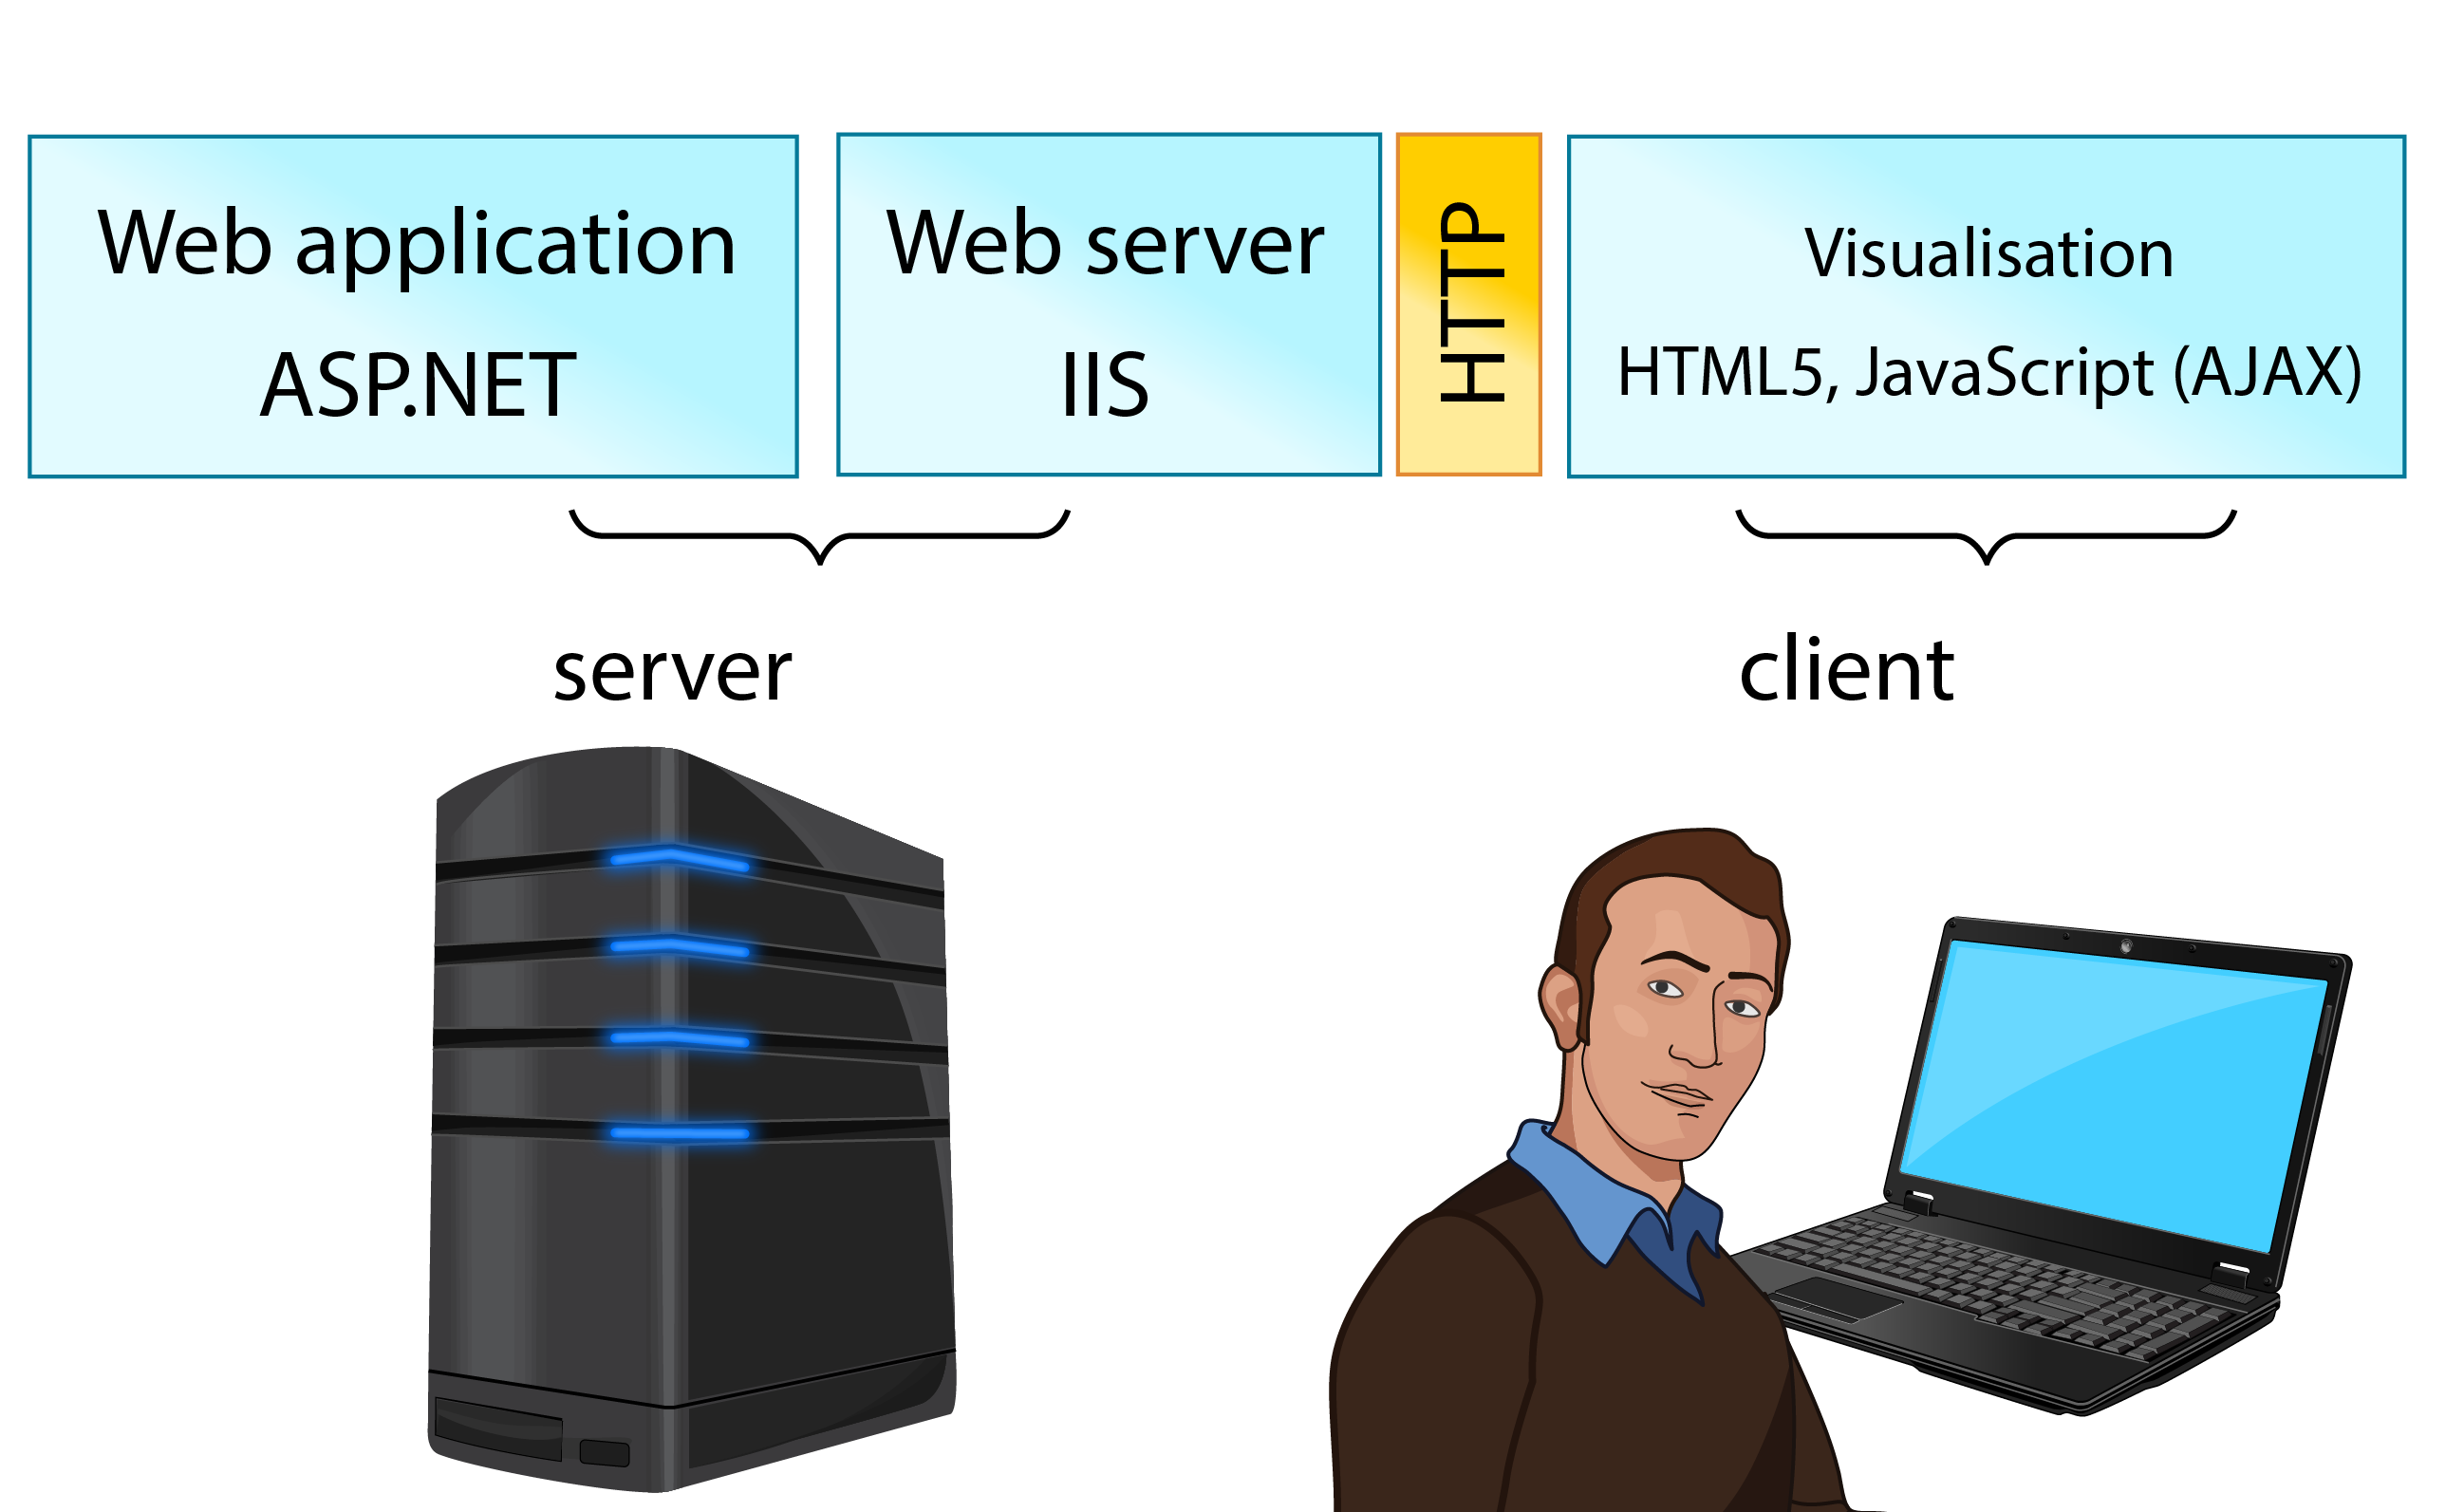
\includegraphics[width=1\textwidth]{img/chapter2-architektura-01.png}
    \caption{Example of client-server architecture involving a web server, which is middleware between web application and server platform. A hypertext document is retrieved from a server via HTTP protocol. Client visualizes a hypertext document in HTML format and may use some interactivity written in Javascript code. Server implementation is in this case realized by Microsoft's Internet Information Server (IIS) and web application is written using ASP.NET server-side Web application framework(\url{http:\\www.asp.net}).}
    \label{fig:architecture}
\end{figure}

%Client-server architecture consist of two and more layers(tiers) E.g. three tier architecture consists of presentation (client) - logic and data tier (server) and each of the server tiers may reside on different physical resources. Example in fig. \ref{fig:architecture}) shows the web server, which is a middleware delivering some abstract functionality expected such as listening on specific TCP/UDP port, call appropriate functionality or deliver a static document, and such middleware is not implemented by the author of the application who deals only with server specific and client specific part. 
%In recent years several architecture styles are applied.

Service-oriented Architecture (SOA)\nomenclature{SOA}{Service-oriented Architecture} is a high-level programming model, which is based on self-contained units of functionality -- service -- and wrapped with documented interfaces. SOA introduces a new layer -- service layer -- in client-server architecture, which separates service interface from its implementation. T. Erl describes further SOA principles and paradigms \cite{Erl2008}. 

Another approach represents the objects and data of a system as resources with a standard set of operations: create, read, update, delete (CRUD)\nomenclature{CRUD}{Create Read Update Delete}. Representation State Transfer (REST)\nomenclature{REST}{Representation State Transfer} specifies several architectural constraints that help scalability and performance. It presents functionality via a fixed number of operations and uniform resource locations (URLs), as proposed by Fielding \cite{fielding2000chapter}. The constraints of REST are:  application is statelessness, resource-orientated with uniform interface (CRUD) and hypermedia-driven, which should facilitate and optimize the processing of resources via current web based technologies, mainly HTTP protocol. 

While SOA focuses on application design and easily turning application objects into distributed services, REST is rather a set of constraints on the architecture, which are used to handle the issues of distribution within the web, as noted by Vinoski \cite{Vinoski2007}.

The software architecture of enterprise applications, distributed systems and some repeating patterns are cataloged in published works, e.g., by Fowler et. al\cite{Fowler2003} or Nilsson \cite{Nilsson2006}. Furthermore, Hohpe et al. disusses integration patterns, with a focus on the ways of connecting heterogeneous parts of the system \cite{Hohpe2002}.
\subsubsection{Types of computing infrastructure}
When we focus on the architecture of middleware and the philosophy of building a computing infrastructure, these main types of distributed infrastructures are distinguished for scientific computing and are relevant to the rest of this work:
\begin{enumerate}
\item{\emph{Service grid computing} is based on the idea that computing resources (servers, clusters and special hardware) are owned by some organizations but may be maintained by some collective organizations and shared with an effort to provide a collection of services in a best effort approach. See section \ref{sec:servicegrid}.}
\item{\emph{Desktop grid computing} is based on the idea of connecting generic desktop computers and providing the idle computation time, e.g., as a screen saver or background process to the projects. See section \ref{sec:desktopgrid}.}
\item{\emph{Cloud computing} provides access to software, platform or whole infrastructure as a service in an elastic way via Internet. The resources are realized using virtualization and provisioned based on the current requirement with minimal administration intervention. See section \ref{sec:introvirtual} and \ref{sec:cloud}.
}
\end{enumerate}

\subsection{Research and education network}
The fundamental part of any distributed computing infrastructure is the computer network, which connects resources that are distributed in different geographical locations, generally on the Internet. 

The national grid initiative in the Czech Republic, METACENTRUM\footnote{\url{http://www.metacentrum.cz}}, is interconnected via the high-speed network, CESNET 2, which utilizes the technology of transferring data over optical cables using Dense Wavelength Division Multiplexing (DWDM)\nomenclature{DWDM}{Dense Wavelength Division Multiplexing} \cite{novak2007deployment}, as seen in Figure \ref{fig:cesnet}.

\begin{figure}[ht]
    \centering
    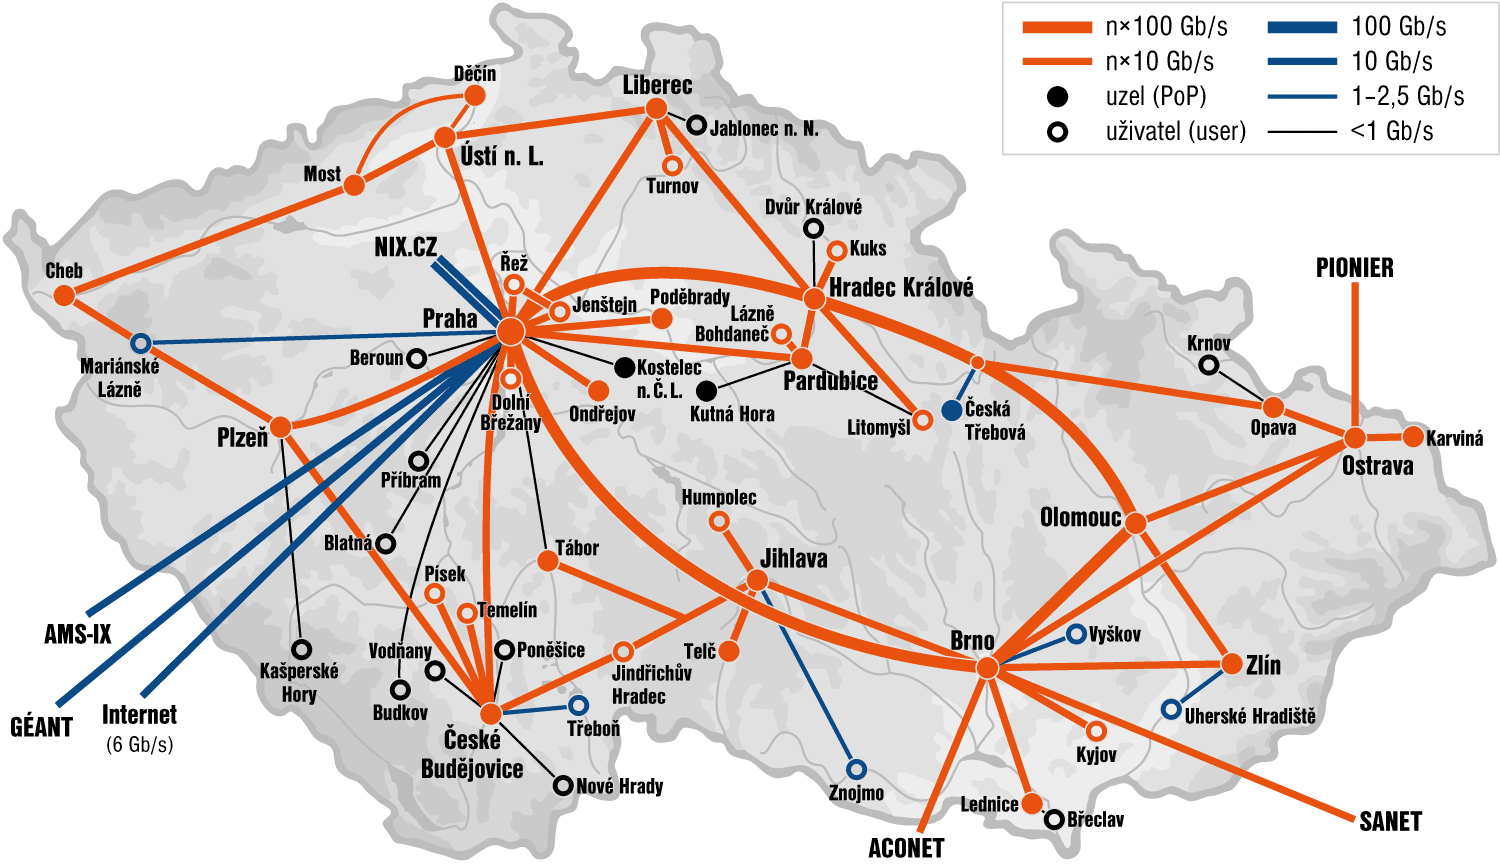
\includegraphics[width=1\textwidth]{chapter2/cesnet2-topo1.png}
    \caption{CESNET2 network topology in December 2014. It has been maintained by association CESNET (association of universities and academy of science in the Czech Republic to operate research and educational network). It mainly interconnects departments of universities and academy of sciences via a rented physical network. It provides connection to the general Internet via the Czech NIX.cz (Neutral Internet eXchange), AMS-IX (Amsterdam Internet eXchange) and European research and education network GÉANT. Sources: \url{http://www.cesnet.cz}}
    \label{fig:cesnet}
\end{figure}

\subsection{Service Grid Computing}
\label{sec:servicegrid}

Service grid computing is based on a basic set of services, which are implemented by a specific grid middleware. They provide uniform interface for job scheduling and execution within the computing infrastructure. The term \emph{grid} is used to emphasize the analogy with an electric power grid, providing access to electricity \cite{foster2004}. Foster et al.\cite{foster2001,foster2004} and Chervenak et al. \cite{Chervenak2000} describe "data" and "computational" grids as shared hardware and software resources, which provide reliable, consistent, pervasive and cheap access to high performance computational capacities. They also provide the effective and reliable execution of requests over data, which needs sensitive controlling of terabyte storage, data transfers to gigabits per second over global computer networks and the scheduling of such data transfer, with respect to computational needs. The services provided by grid are either tools or web services, following  \emph{Service Oriented Architecture} (SOA) for grid computing -- Open Grid Service Architecture (OGSA)\nomenclature{OGSA}{Open Grid Service Architecture} \cite{Foster2003}. The security model and access to grid infrastructures are mainly proposed and implemented by a mutual authentication between users and resources via a public key infrastructure, using the X.509 certificate \cite{Foster1998}.
\begin{figure}[htb]
    \centering
    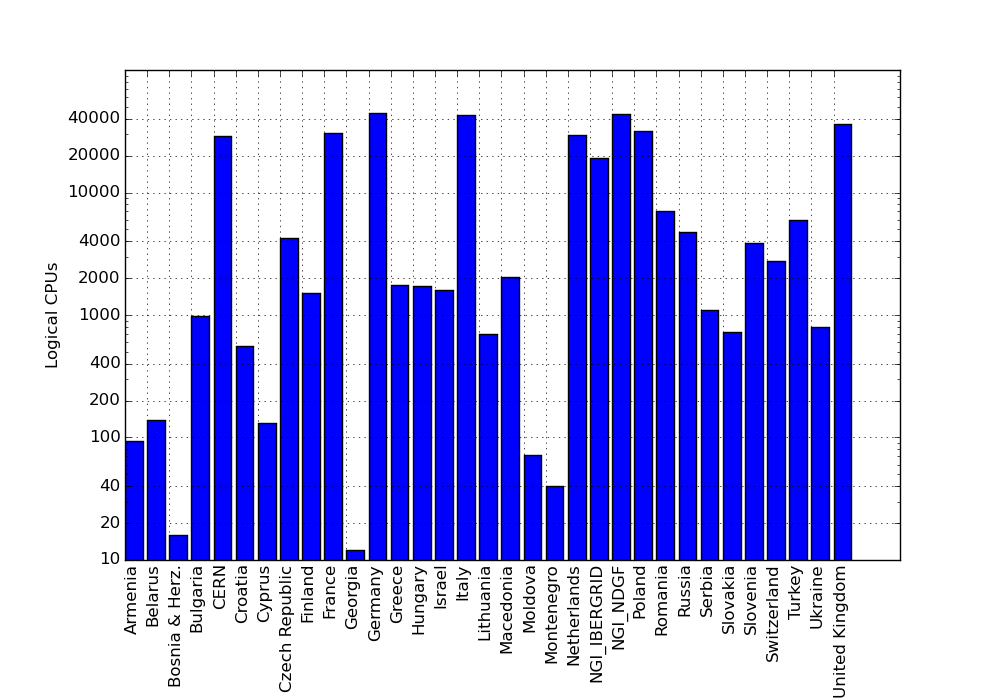
\includegraphics[width=0.9\textwidth]{chapter2/egicpus.png}
    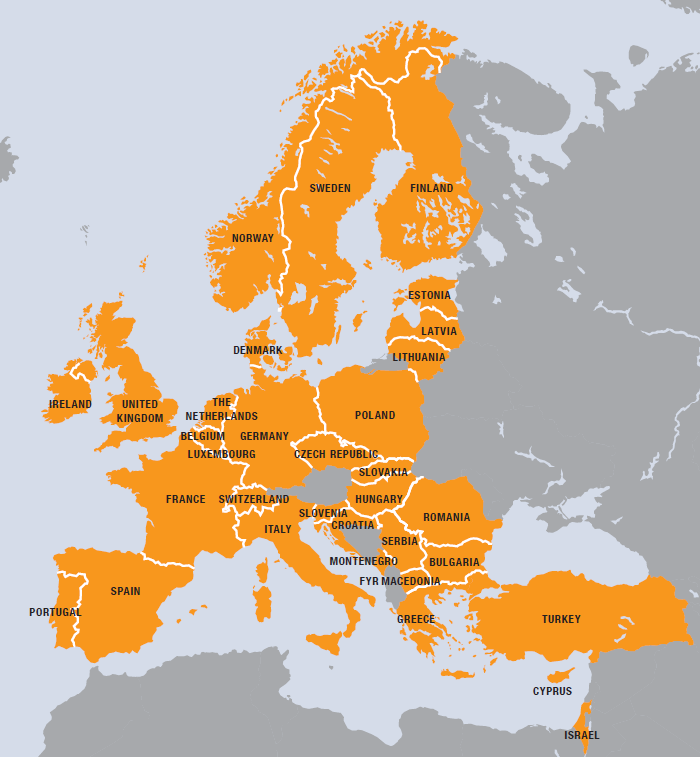
\includegraphics[width=0.7\textwidth]{chapter2/egi.png}
    \caption{Countries involved in EGI and number of CPUs within EGI infrastructure in 2012, the total logical CPU capacity at the end of 2012 was 349~720 cores( in graph per countries). CPU capacity was 433~957 cores in March 2014. Sources: EGI Compendium 2013, EGI statistics at \url{http://www.egi.eu}.%\bibentry{EGICompendium2013} \bibentry{egi2014}.
    }
    \label{fig:egi}
\end{figure}
The administration and maintenance of such networked infrastructures are not trivial tasks and are performed by experts of institutional computing centers or national laboratories. Furthermore, interconnected sites are managed and coordinated at a national level or an international level. Such national organizations cooperate with similar national grid infrastructures in other countries. An umbrella organization in Europe -- the European Grid Infrastructure (EGI)\nomenclature{EGI}{European Grid Infrastructure}\footnote{\url{http://www.egi.eu}} -- was established during 2010. It supports the integration and coordination of activities of national grid initiatives (NGI)\nomenclature{NGI}{National Grid Initiative}. Countries connected to the EGI and approximate number of CPUs per country in 2014 are presented in Figure \ref{fig:egi}.

In the last decade, there has been an acceleration in the growth of several production grid infrastructures for science. This is mainly due to the need for experiments of high-energy physics in order to process a large number of observed data in a reasonable time \cite{Bird2009}. The Worldwide Large Hadron Collider Computing Grid (WLCG)\nomenclature{WLCG}{Worldwide Large Hadron Collider Computing Grid} was designed to store and process almost 30 PetaBytes of data per year in the period of 2009-2013  \cite{Adamova2014}. It is one of the largest grids to be deployed in a grid infrastructure. As the hardware infrastructure is built with a philosophy of federated access to resources, which are owned by research institutions, universities, etc. Other scientists from different scientific disciplines can also become users of this powerful infrastructure. Due to the development of virtualization, the infrastructure can employ a larger set of applications and services and could be attractive for smaller scientific collaboration with different requirement on platform, shared libraries, etc.

Several grid infrastructures were established, based on different grid middlewares.
Condor is one of the earliest efforts to provide access to underutilized computers, while preserving the rights of the owners \cite{Litzkow1990}. Major grid middlewares that are operational in EGI are Globus \cite{Foster1997}\footnote{\url{http://toolkit.globus.org/toolkit/} accessed February 2015}, gLite \cite{Laure2006}\footnote{\url{http://glite.cern.ch} accessed February 2015} and ARC\footnote{\url{http://www.nordugrid.org/arc/} accessed February 2015}.

Efforts are currently being made to maintain interoperability in order to connect different applications with different resources from different grid infrastructures. Riedel et al. reports on the efforts being made to involve technology providers, as well as deployment teams, in order to participate in open standards of security, data management, etc. \cite{Riedel2009}.

\subsection{Desktop Grid Computing}
\label{sec:desktopgrid}
Joining desktop computers from an individual user to form a voluntary or desktop grid was popularized by a project that tries to identify uncommon signals from space to search for extraterrestrial intelligence (SETI@Home)\footnote{\url{http://setiathome.ssl.berkeley.edu/}}. It is based on the idea that a volunteer downloads a small client program, which executes in the background or instead of a screen saver. It downloads additional data from a server on the Internet in order to be analyzed. It then sends the results back to the server. In contrast to service grids, the authorization of users cannot be so strong for volunteer individuals and some other policies, e.g., redundancy and validation, are implemented to eliminate bad or cheating results \cite{Anderson2002}. After the success of the SETI@Home, general-purpose frameworks were built in order to facilitate the development of projects that use a similar philosophy of computing on desktop computers, which are connected via the Internet such as BOINC\nomenclature{BOINC}{Berkeley Open Infrastructure for Network Computing} \cite{Anderson2004}, SZTAKI extension to BOINC \cite{Balaton2007,Kacsuk2009}, XtremWeb \cite{Fedak2001} and others. Currently, there are a lot of similar projects that gain the same computer power as the SETI@Home project, e.g., the LHC@Home and it's successor, LHC@Home 2. These projects were established and used to execute  selected tasks to analyze data from the Large Hadron Collider (LHC)\nomenclature{LHC}{Large Hadron Collider} project \cite{Herr2006,Hoimyr2012}.

The average performance of BOINC projects is 8.073 PetaFLOPS,  with 294~764 volunteers computing on 502~238 computers (March 18$^{th}$ 2015). For example SETI@Home's 24 hour performance is 1.95 PetaFLOPS. Although desktop grids and service grids are two different approaches that are used to gather computing power from a large number of computing resources, efforts are being made to interoperate and share the capacity among infrastructures, e.g., the EdgE project, published by Kacsuk et al.\cite{Kacsuk2008}  and Urbah et al. \cite{Urbah2009}.

\subsection{Virtualization}
\label{sec:introvirtual}
Virtualization technology separates the physical hardware layer from the software environment, emulating a new virtual hardware layer. The hypervisor (or virtual machine manager) manages guest virtual machines and translates I/O\nomenclature{I/O}{Input Output} operations between virtual device and physical device. It also translates instructions from virtual CPU to physical CPU. This introduces some overhead and performance degradation of virtual system compared to physical. However, recent virtualization technology has introduced several techniques that reduce overhead and eliminate specific hardware features and instructions which are hard to virtualize, as reported by Barham et al. and Youseff et al. \cite{Barham2003,Youseff2006}.
Thanks to them, a virtual environment has been fine-tuned for an application that can be executed on almost any hardware and platform. Here, virtualization becomes part of the solution to execute jobs of desktop grid or service grid projects on different physical platforms, as published, e.g., by Ruda et al. \cite{ruda2009virtual}.
Currently, there are several commercial, free or even open-source virtualization implementations, which are provided by different vendors and hypervisors - VMWare\footnote{\url{http://www.vmware.com/} accessed March 2015}, XEN\footnote{\url{http://www.xenproject.org/} accessed March 2015}, KVM\footnote{\url{http://www.linux-kvm.org/} accessed March 2015}, VirtualBox\footnote{\url{https://www.virtualbox.org/} accesse March 2015} etc. 


\subsection{Cloud Computing}
\label{sec:cloud}
In contrast to grid computing, where a user schedules jobs in order to access shared environment and may be influenced by other users or by the environment, cloud computing provides access to a virtual software, platform or whole infrastructure. Consequently, the user or process is given the impression of sole use. Virtualization techniques have enabled expansion of cloud computing, mainly on infrastructures that were built for another purpose. These can be rented in times when the primary infrastructure is not fully utilized \cite{Foster2008}. 
%changes 28th march
Typically, the access to shared computing resources can be rapidly provisioned and released with minimal management effort or service provider interaction. This implicates other important feature of cloud-computing -- elasticity -- ability to scale up and down computing resources when required. These and other characteristics were collected and published by Mell and Grance in the NIST definition of cloud computing \cite{Mell2011}.
%Cloud-computing can be characterized as a model for enabling ubiquitous, convenient, on-demand network access to a shared pool of configurable computing resources (e.g., networks, servers, storage, applications, and services) that can be rapidly provisioned and released with minimal management effort or service provider interaction \cite{Mell2011}.  

Cloud computing makes computational power and storage as utilities or commodities that can be rented. With current commercial clouds, the commercial area has evolved in order to facilitate scaling up per the business needs and computational demand, e.g., Amazon EC2\footnote{\url{http://aws.amazon.com/ec2/} accessed February 2015}, Microsoft Windows Azure \footnote{\url{http://azure.microsoft.com/} accessed February 2015}, Google cloud\footnote{\url{https://cloud.google.com/} accessed February 2015} and others.
 
Cloud computing is provided in several fundamental models or categories. Infrastructure as a Service (IaaS)\nomenclature{IaaS}{Infrastructure as a Service} offers the whole virtual infrastructure including virtual machine and network. User can install operating system images and application software. Platform as a Service (PaaS)\nomenclature{PaaS}{Platform as a Service} offers a specific computing platform including development tools, programming language, libraries and databases. User can use PaaS to develop and execute his own domain-specific application. Software as a Service (SaaS)\nomenclature{SaaS}{Software as a Service} offers access to a final software, usually in a form of web application. User can use SaaS with web-browser or with some specific client software.
Cloud computing in research infrastructures is being deployed next to the already existing grid infrastructures and can utilize the same hardware resources. Some methods to integrate grid computing and cloud computing was proposed, e.g., with PaaS approach by Anjum et al. \cite{Anjum2012}, or with a plugin for existing grid portal by Kacsuk \cite{Kacsuk2011}. Currently, the most used platforms are Open\-Nebula  \cite{Milojicic2011} and OpenStack \cite{Kumar2014} in research infrastructures. Interoperability among cloud providers and a standardization of cloud computing, virtualization and related technologies are important as these would keep users from being locked into a specific cloud provider, as noted by Otiz \cite{Ortiz2011}.

\subsection{Application Model}

Applications that are computed within a grid or cloud infrastructure can be characterized by the quantity of tasks being performed, the size of the input data and the communication that needs to be carried out between concurrent tasks. 
Grid computing infrastructures are primarily utilized for computation, in which tasks take a long time. These are relatively loosely coupled and resources are used over a long period of time. Performance or capacity is usually mentioned  in operations or CPUs per month or year and for such computations, the term High throughput computing (HTC)\nomenclature{HTC}{High Throughput Computing} is used.

%While HTC takes a long time, 
The High Performance Computing (HPC)\nomenclature{HPC}{High Performance Computing} is usually characterized by computing problems that have a small number of tasks. These are relatively tightly coupled and can take shorter time than HTC. Performance is measured in operations per second (FLOPS)\nomenclature{FLOPS}{Floating-Point Operations per Second} \cite{Hager2010,Levesque2010}. The grid infrastructure can involve HPC servers or clusters.% and, thus, a job or task that requires such HPC hardware is scheduled and executed there.

Many Task Computing (MTC)\nomenclature{MTC}{Many Task Computing} aims to bridge HTC and HPC. While the computation usually takes a shorter amount of time, the data exchange is in MB rather than in GB. Performance is measured in tasks per seconds rather than jobs per months or years and it involves computing much more heterogeneous problems, which are not "happily" parallel. %However, middleware for HPC or HTC, which are present in grid computing infrastructures, may introduce some shortcomings. 
Therefore Raicu et al. proposed and implemented a prototype of task execution framework, which is suitable for MTC to prevent some shortcomings of HTC or HPC \cite{Raicu2008, Raicu2009,Raicu2010}.
%MTC seems suitable fore performance on cloud computing technologies, however, such clouds should be oriented for HPC systems and a generic public cloud may introduce a lower performance than expected \cite{Iosup2010}.

\subsection{Workflows and Gateways}
\label{sec:introworkflow}
A workflow is an abstract description of the process of computation and data manipulation, which is  specified by an expert in order to express what should be done within a distributed system. It automates the process of computation by composing data manipulation steps and tasks, as well as solving failures.

The workflow can be encoded in any programming or scripting language, however, some higher level languages have evolved. In the business domain, a Business Process Execution Language (BPEL)\nomenclature{BPEL}{Business Process Execution Language} has become one of the most used languages for describing the workflow of orchestration of web services and transaction steps \cite{Pasley2005}. In the scientific domain, different workflow systems are operational, including BPEL, with different capabilities. Yu, Zhao et al. published the taxonomies of some of the existing workflow systems \cite{Yu2005a,Zhao2008,Curcin2008}. Workflows in cloud computing can be covered also by web technologies programming languages, e.g., Javascript \cite{Foster2008}.

The workflow system, which implements concrete workflow language, is usually tightly coupled with a specific grid computing or cloud computing infrastructure. 

To connect the different grid infrastructures, a mutual workflow management system can be used to integrate them, as proposed by Kacsuk et al. \cite{Kacsuk2008a,Kacsuk2011}.% Interoperability is solved by separating the abstract workflow representation and concrete implementation, which are shown on the selected existing workflow systems introduced by Planensteiner et al. \cite{Plankensteiner2013}.

Scientific gateways incorporate a higher level of services for specific scientific communities, e.g., a web portal or desktop application in order to control the process of computation via a workflow\cite{Wilkins-Diehr2007}. Several frameworks were developed for building scientific gateways, e.g., Apache Airavata \cite{Pierce2014,Memon2014} or WS-PGRADE/gUSE\cite{Kacsuk2012}. Furthermore, the concrete instances are available for a broader area of the scientific community. 


%\section{Informatics in Medicine and Biology}
%\label{sec:biology}

